\section{Simulación del sistema sin atascamiento-deslizamiento}

En base a la revisión de modelos, se decidió adoptar el modelo que ha sido ampliamente estudiado en la práctica, específicamente en el artículo y la tesis de Diana, los cuales han sido referenciados en otros trabajos de investigación y han sido respaldados con experimentos reales.

La realización en espacio de estados para el caso inestable es:

\begin{itemize}[label={}]
    \item{ 
    \begin{align*}
        &F_{em}= \dfrac{u}{b(a-x_{1})^4} 
    \end{align*}

    }   
\end{itemize}
La fuerza electromagnética se expresa como una función de cuarto grado que depende directamente del voltaje de control e inversamente de la distancia. Los parámetros $a$ y $b$ son obtenidos experimentalmente, siendo $x_{1}$ la distancia entre el electroimán superior y el disco ferromagnético.\cite{maaz}\cite{naz}

Al recurrir a este modelo específico, se busca aprovechar los avances y conocimientos generados por la comunidad científica en torno a su diseño y rendimiento. Su elección se respalda tanto en la investigación académica como en la experiencia práctica, lo cual brinda una mayor confianza en su efectividad y resultados.

\section{Modelo en configuración inestable}

En el ámbito de la literatura especializada, hasta el momento no se ha tratado de manera completa un problema que involucra el fenómeno del atascamiento-deslizamiento inestable. Dado que no se ha explorado ni comprendido a fondo, es crucial abordar este problema para expandir nuestro entendimiento.

En este sentido, nos proponemos dirigir nuestra atención hacia el sistema del levitador en una configuración específica y particularmente inestable. Cabe destacar que se ha reportado la aparición de este fenómeno en un artículo y una tesis elaborados por Diana, los cuales proporcionan información valiosa sobre el tema.


\setboolean{image}{false} 
\ifthenelse{\boolean{image}}{
    \begin{figure}[htbp]
        \centering
        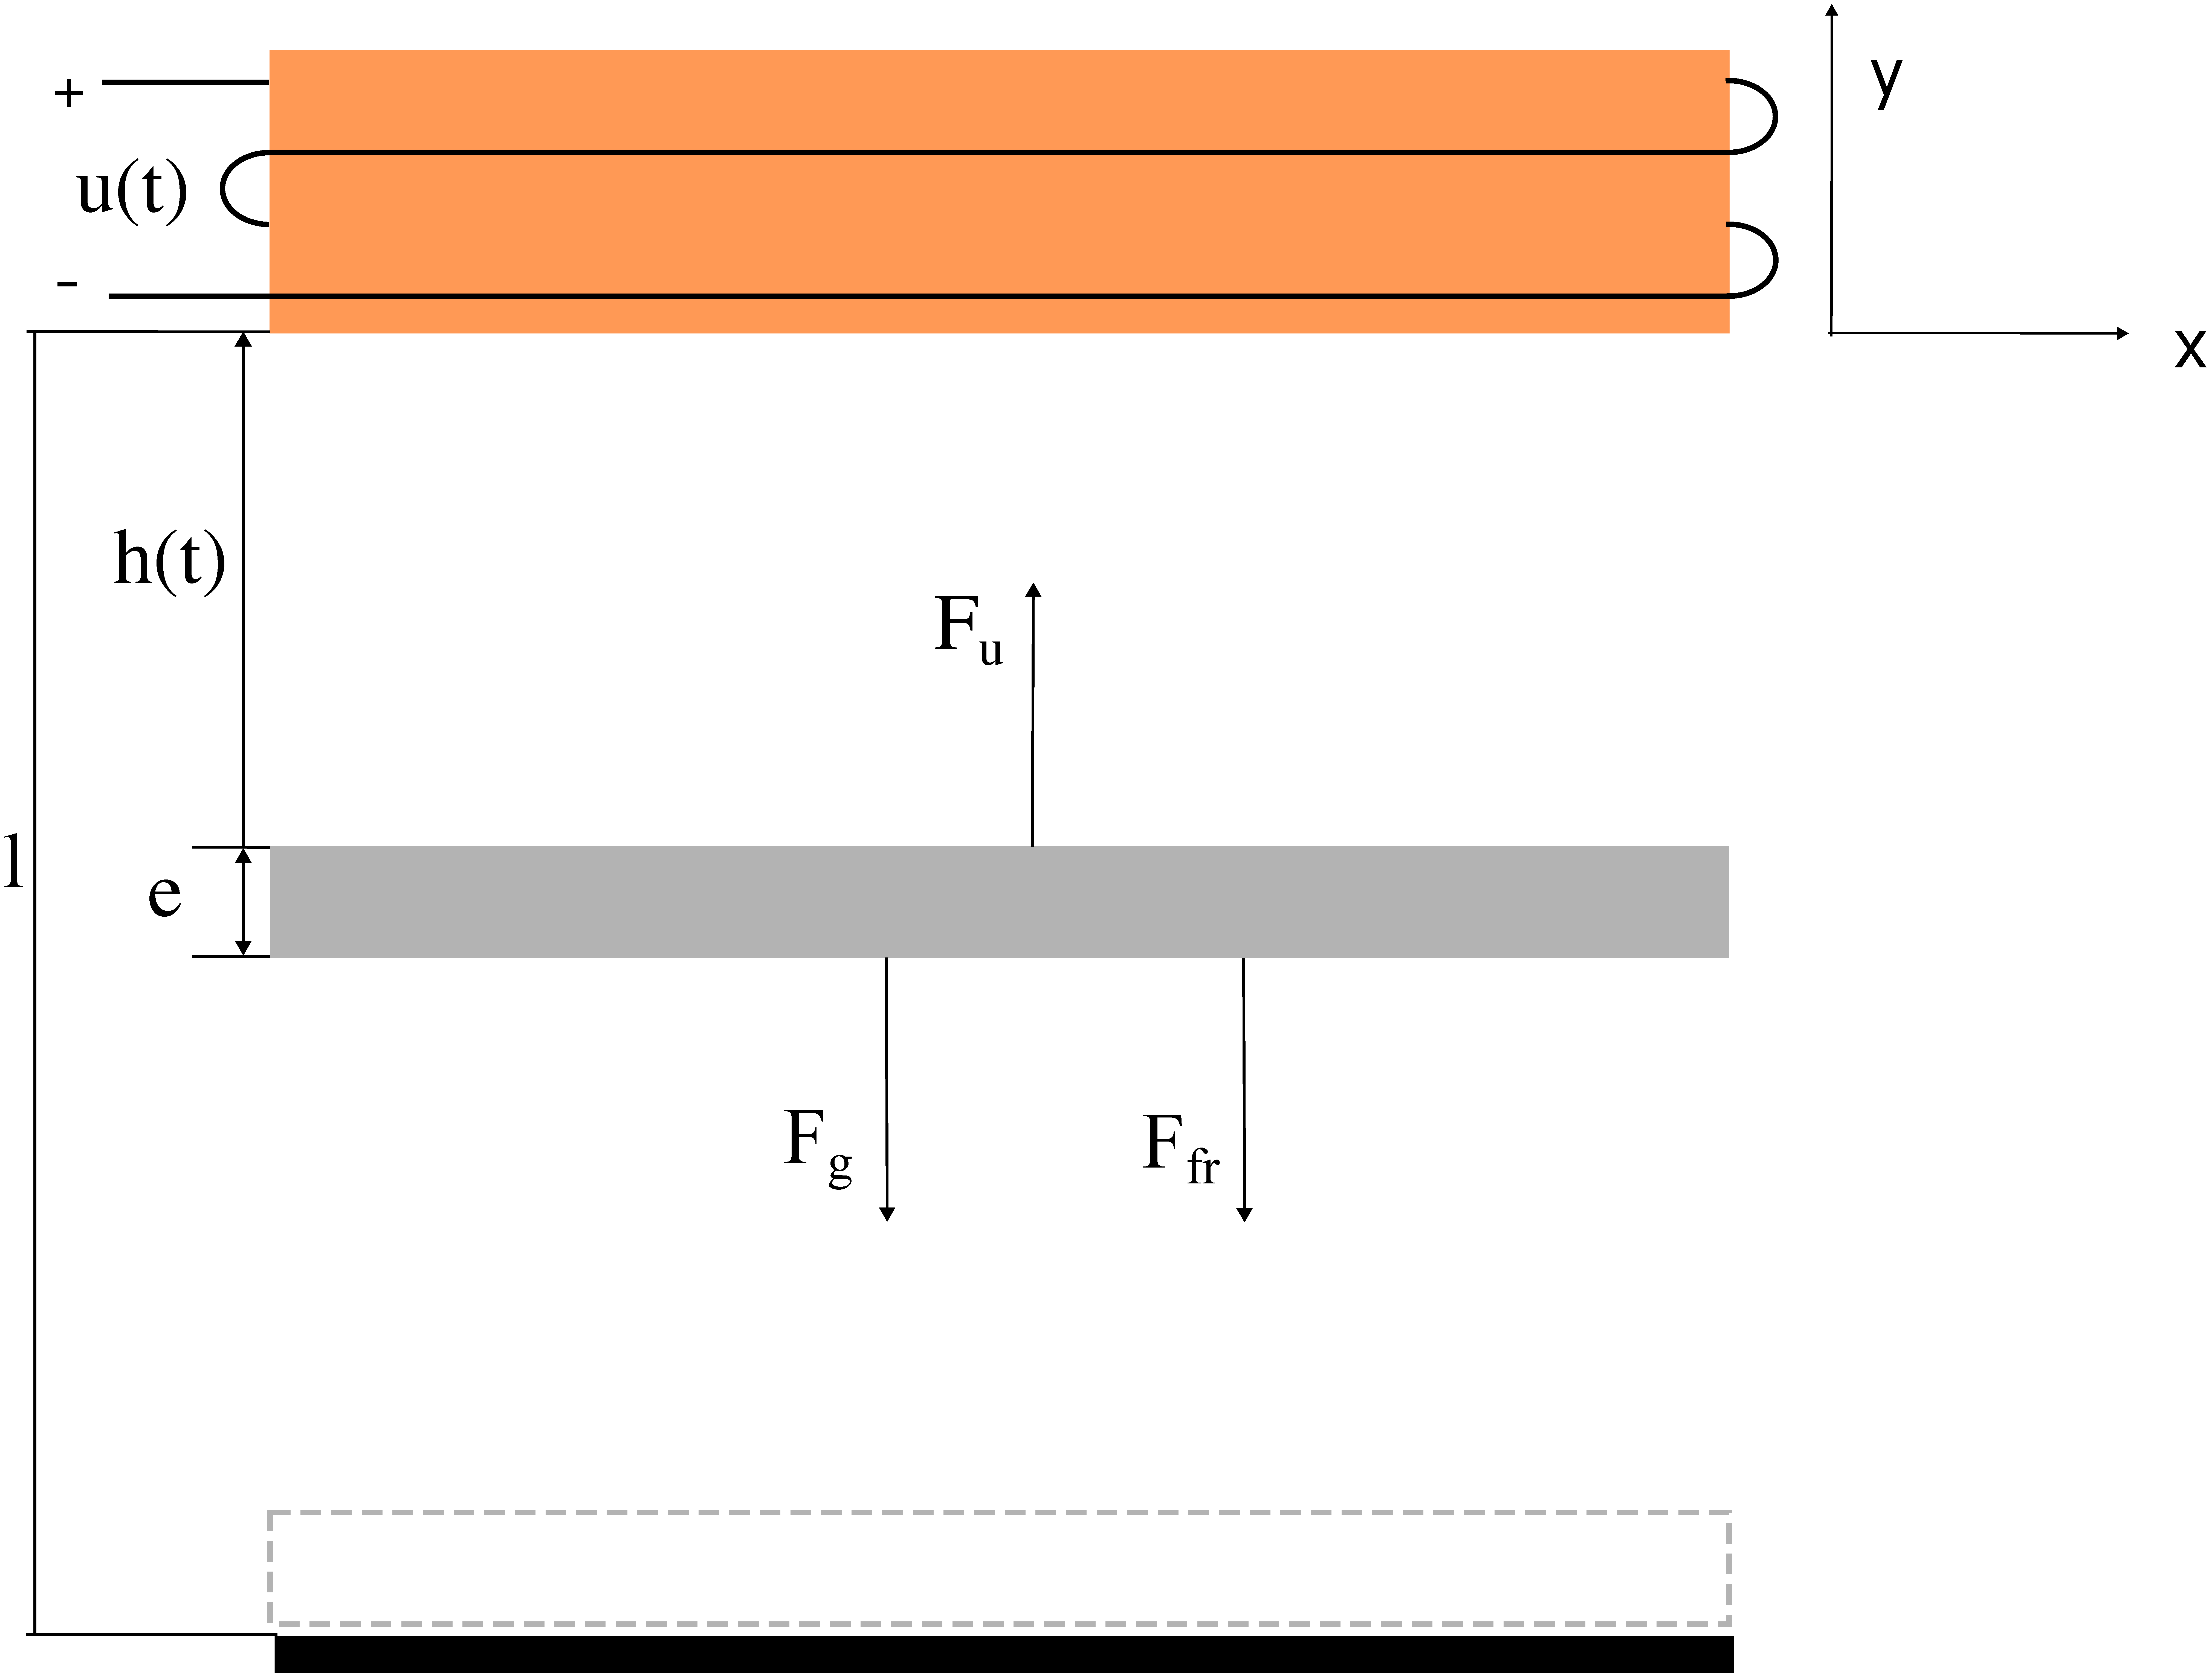
\includegraphics[width=0.5\textwidth]{images/configurations/configuracion_inestable.eps}
        \caption{SLM en configuración inestable}
        \label{fig:SLMinestable}
    \end{figure}
}{
    \begin{figure}[htbp]
        \centering
            \fbox{%
                \begin{minipage}[c][1in][c]{1in} 
                    \centering % Center the text
                    Your text here
                \end{minipage}%
            }
        \caption{SLM en configuración inestable}
        \label{fig:fbox}
    \end{figure}
}


Sin embargo, nos enfrentamos a un desafío significativo debido a la indisponibilidad del equipo requerido para llevar a cabo experimentos directos. Afortunadamente, contamos con una alternativa viable para abordar esta limitación: la simulación. Por lo tanto, hemos optado por realizar un estudio exhaustivo y detallado utilizando técnicas de simulación que nos permitirán explorar y comprender los aspectos fundamentales del fenómeno de atascamiento-deslizamiento inestable en el sistema del levitador.

Al emplear esta metodología, buscamos obtener resultados concluyentes y fiables que contribuyan a llenar el vacío existente en la literatura y aporten una perspectiva más amplia sobre este problema particular. Además, esta aproximación nos permitirá evaluar diferentes escenarios y condiciones de manera controlada, brindándonos una mayor comprensión de los factores que influyen en el fenómeno y sus posibles implicaciones prácticas.

Se tuvieron en cuenta como consideraciones iniciales  considerar la fricción lineal. La elección de la zona muerta dura fue seleccionada debido a su capacidad de proporcionar un contraste más sólido con la realidad.


\setboolean{image}{false}
\ifthenelse{\boolean{image}}{
    \begin{figure}[htbp]
        \centering
        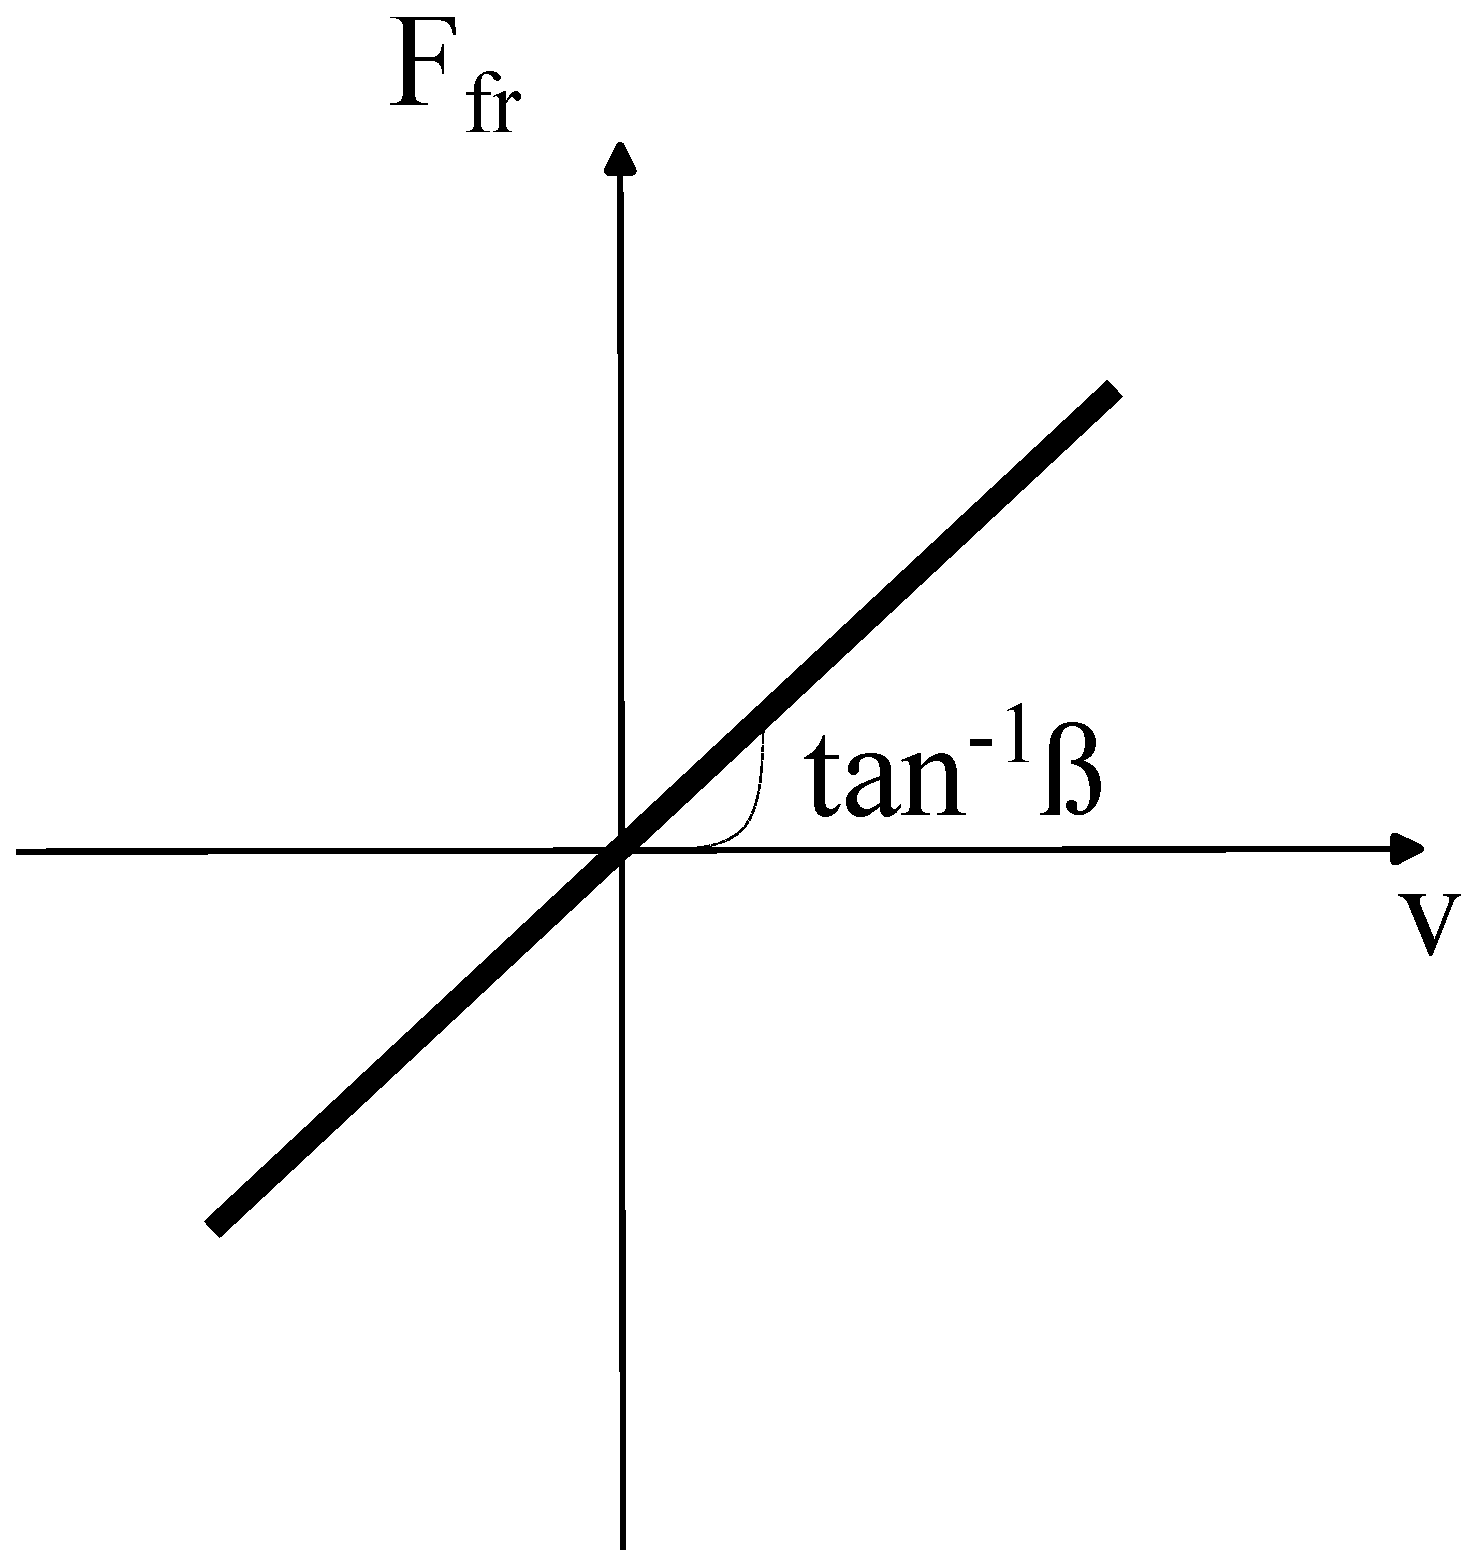
\includegraphics[width=0.3\textwidth]{images/zm_fricc/friccionlineal.eps}
        \caption{Fricción lineal}
        \label{fig:friccionlineal}
    \end{figure}
}{
    \begin{figure}[htbp]
        \centering
        \fbox{%
            \begin{minipage}[c][1in][c]{1in}
                \centering
                Your figure here
            \end{minipage}%
        }
        \caption{SLM en configuración inestable}
        \label{fig:fbox}
    \end{figure}
}


Hay que tener en cuenta que en los levitadores magnéticos, tanto su versión estable como la inestable, la zona muerta es dinámica y está en función del voltaje y la velocidad de equilibrio.


\setboolean{image}{false}
\ifthenelse{\boolean{image}}{
\begin{figure}[htbp]
  \begin{minipage}[b]{0.35\linewidth}
    \centering
    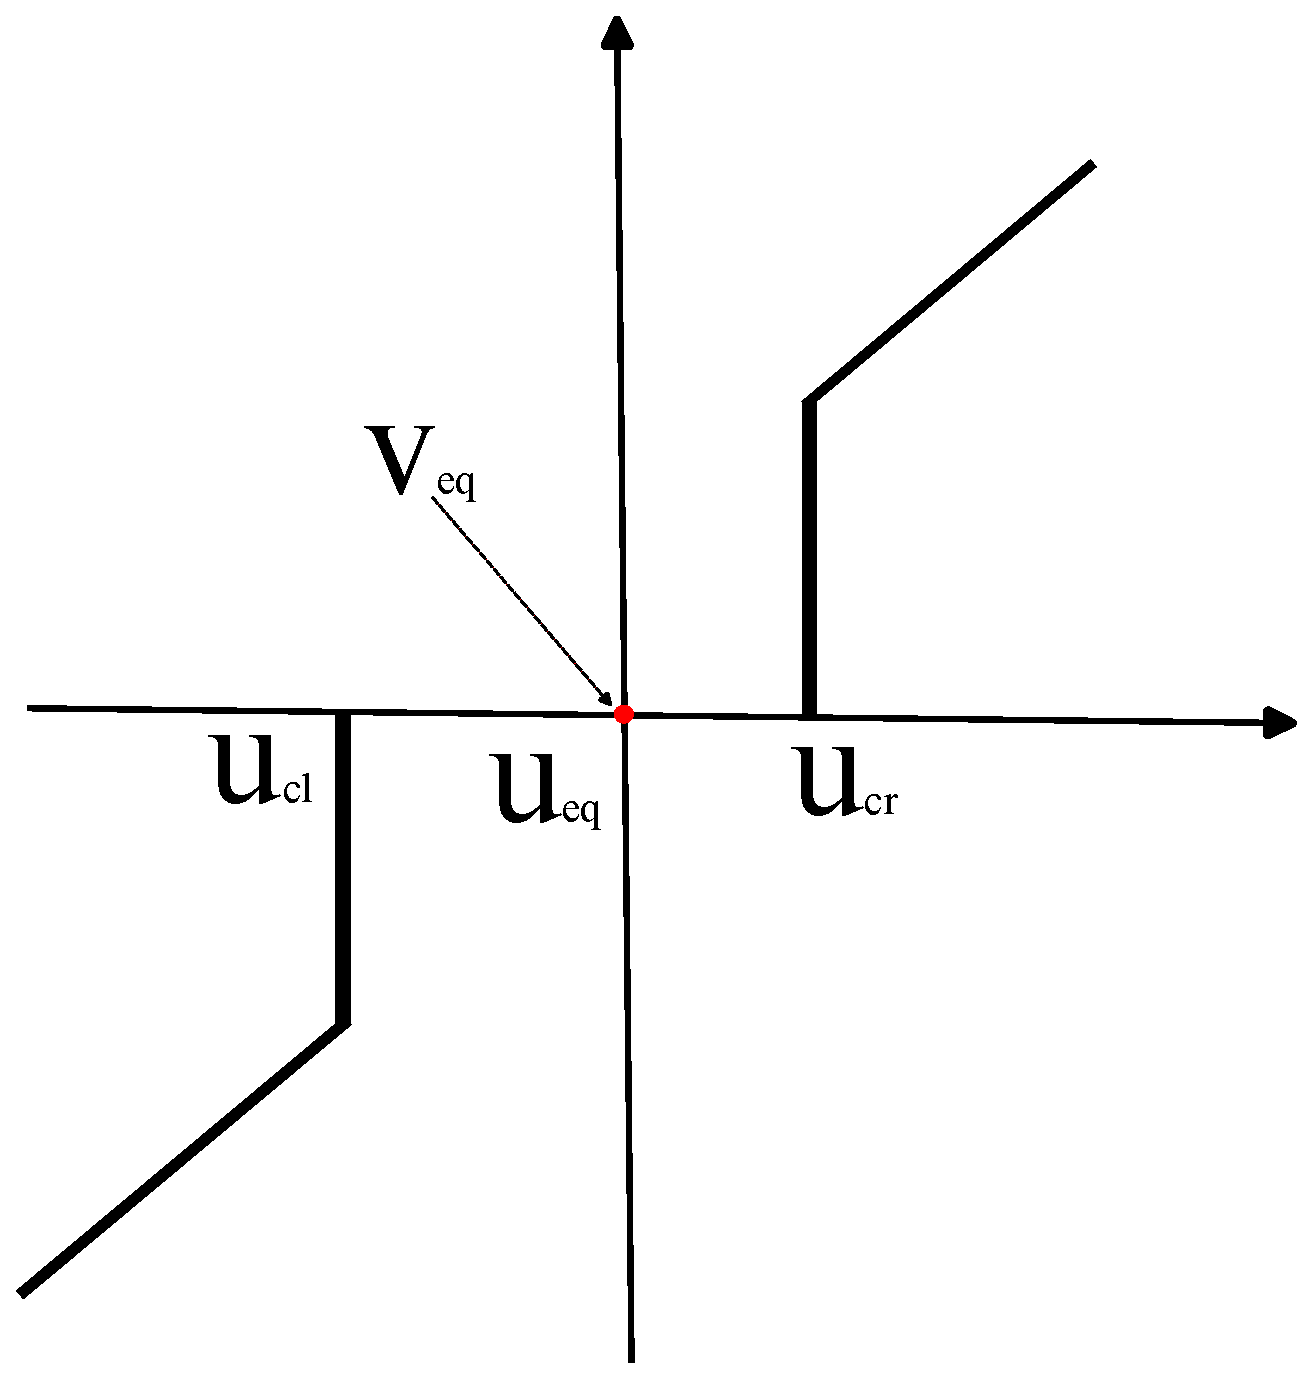
\includegraphics[width=\linewidth]{images/zm_fricc/zm_estatica.eps}
    \caption{Zona muerta estática}
    \label{zmestatica}
  \end{minipage}%
  \hspace{0.2\linewidth} % Aumenta el espacio horizontal
  \begin{minipage}[b]{0.4\linewidth}
    \centering
    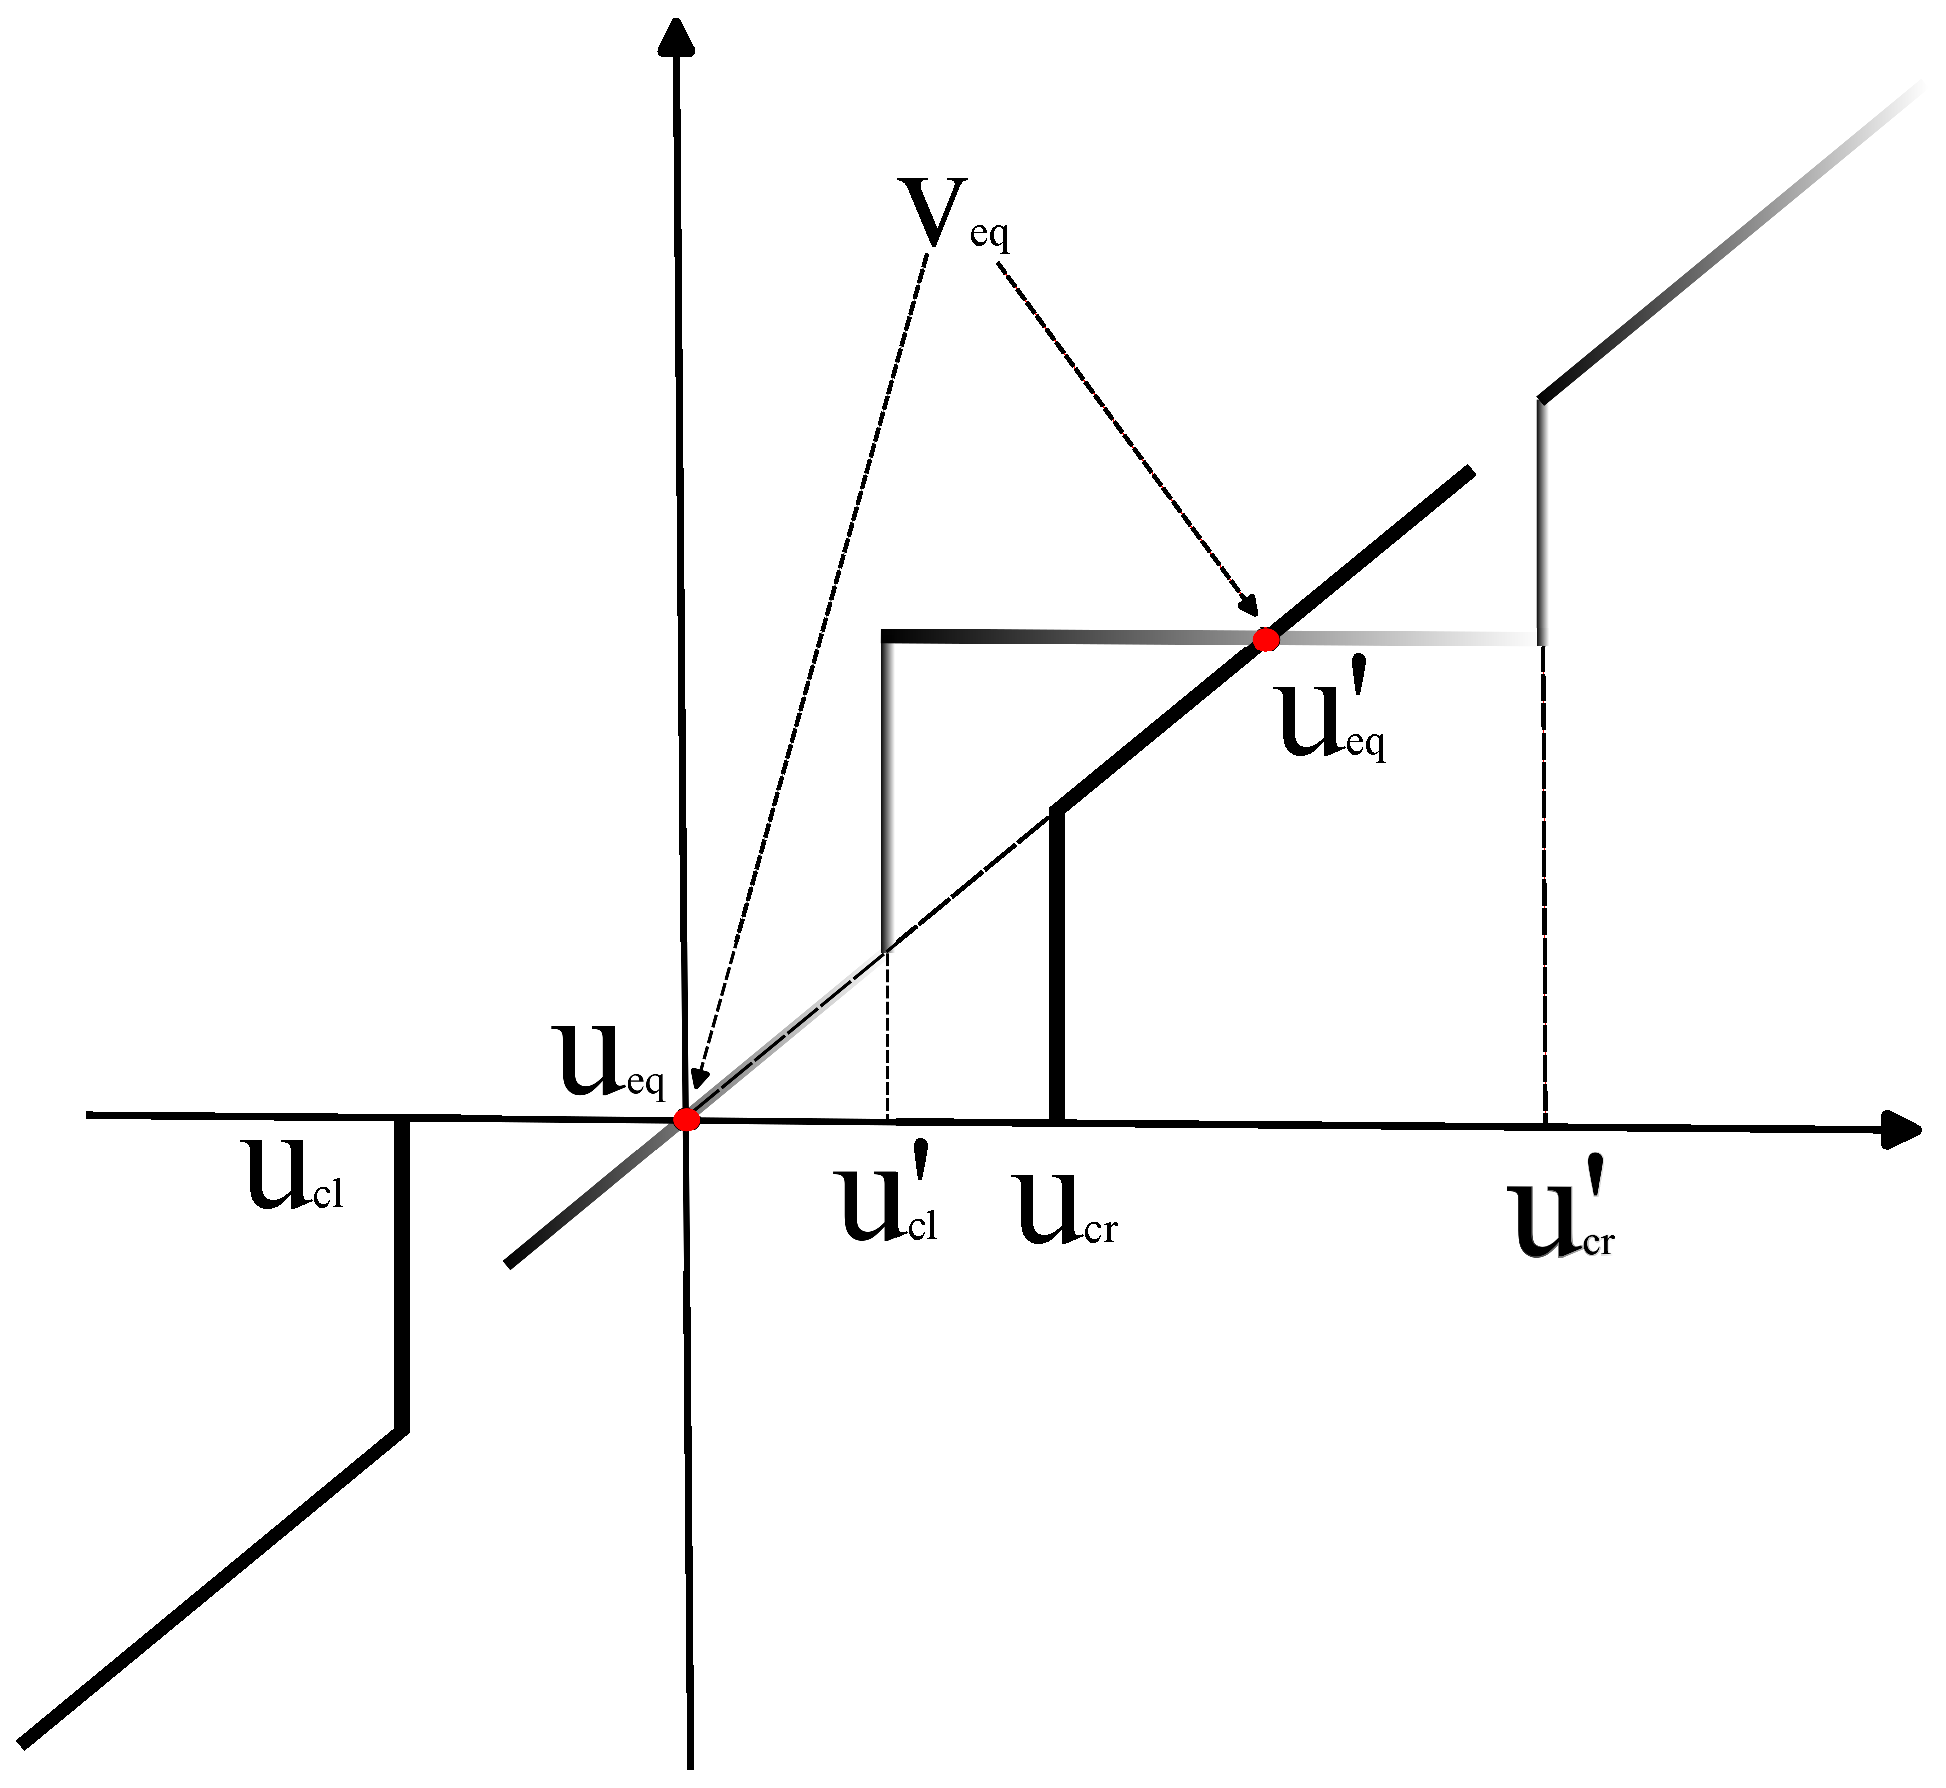
\includegraphics[width=\linewidth]{images/zm_fricc/zm_dinamica.eps}
    \caption{Zona muerta dinámica}
    \label{zmdinamica}
  \end{minipage}
\end{figure}
}{
    \begin{figure}[htbp]
        \centering
        \fbox{%
            \begin{minipage}[c][1in][c]{1in}
                \centering
                Your figure here
            \end{minipage}%
        }
        \caption{SLM en configuración inestable}
        \label{fig:fbox}
    \end{figure}
}

Tomando como referencia el diagrama de cuerpo libre y aplicando la segunda ley de Newton, el sistema de ecuaciones queda como:

\begin{equation}
m\ddot{y}_{(t)}=F_{u}-F_{g} -F_{fr}
\end{equation}

Donde $F_{u}$ es la fuerza del electroimán, $F_{g}$ es la fuerza de gravedad y $F_{fr}$ la fuerza de fricción.

La fuerza magnética puede ser modelada para el caso inestable como:
\begin{equation}
F_{u}=\dfrac{u}{b[a-y_{(t)}]^4}\
\end{equation}

De (1) y (3), la ecuación no lineal de movimiento resulta para el sistema inestable:
\begin{equation}
\ddot{y}_{(t)}=\dfrac{u}{bm[a-y_{(t)}]^4}-c_{1}\dot{y}_{(t)}-g
\end{equation}

con $c_{1}=c/m.$\\
Donde $m$ es la masa del imán en \si{\kilogram}, $y$ es la distancia en \si{\centi\meter} entre la bobina y el centro del imán, $c$ es el coeficiente de fricción, $g$ es la aceleración de la gravedad en $\text{cm/s}^2$, $a$ y $b$ son constantes con unidades de $\text{cm}$ y $\text{V}/(\text{N} \cdot \text{cm}^4)$, respectivamente, y $u$ es el esfuerzo de control en volts.
Adicionalmente, en este caso se consideró que el sistema de levitación magnética está bien diseñado, lo que tiene como consecuencia que la dinámica eléctrica responde más rápido, y por tanto, puede ser despreciada.
